\section{Arquitectura del sistema (pipeline)}
Aquest apartat descriu l'arquitectura del sistema que s'ha desenvolupat per a l'anàlisi automàtica dels tiquets d'incidències de ciberseguretat de l'\textbf{Agència}. L'arquitectura del sistema està encadenada a les màquines que disposem propietat de l'agència i al sistema que en producció en aquests moments. L'\textbf{Agència} ha posat a disposició del equip tres servidors idèntics per cada secció on estaran les dades i dos portàtils amb accés als servidors a través d'una VPN privada.

\begin{itemize}
     \item \textbf{Servidor 1 (OTRS):} Servidor on s'emmagatzema la base de dades d'OTRS amb els tiquets al seu interior.
     \item \textbf{Servidor 2 (Pipeline):} Servidor encarregat d'accedir als altres servidors per llegir i guardar informació i passar-la pel programa desenvolupat per resoldre el problema.
     \item \textbf{Servidor 3 (Elasticsearch):} Servidor que recull les dades processades i anonimitzades per un futur us.
\end{itemize}

\begin{itemize}
     \item \textbf{Portàtil 1 (amb GPU):} Portàtil amb la funció principal d'entrenar el model que serà utilitzat per extreure l'informació dels tiquets. Està configurat per evitar cap bretxa de dades.
     \item \textbf{Portàtil 2 (sense GPU):} Portàtil amb la capacitat d'accedir al servidors de l'\textbf{Agència} mitjançant una VPN.
\end{itemize}

\begin{figure}[H]
     \centering
     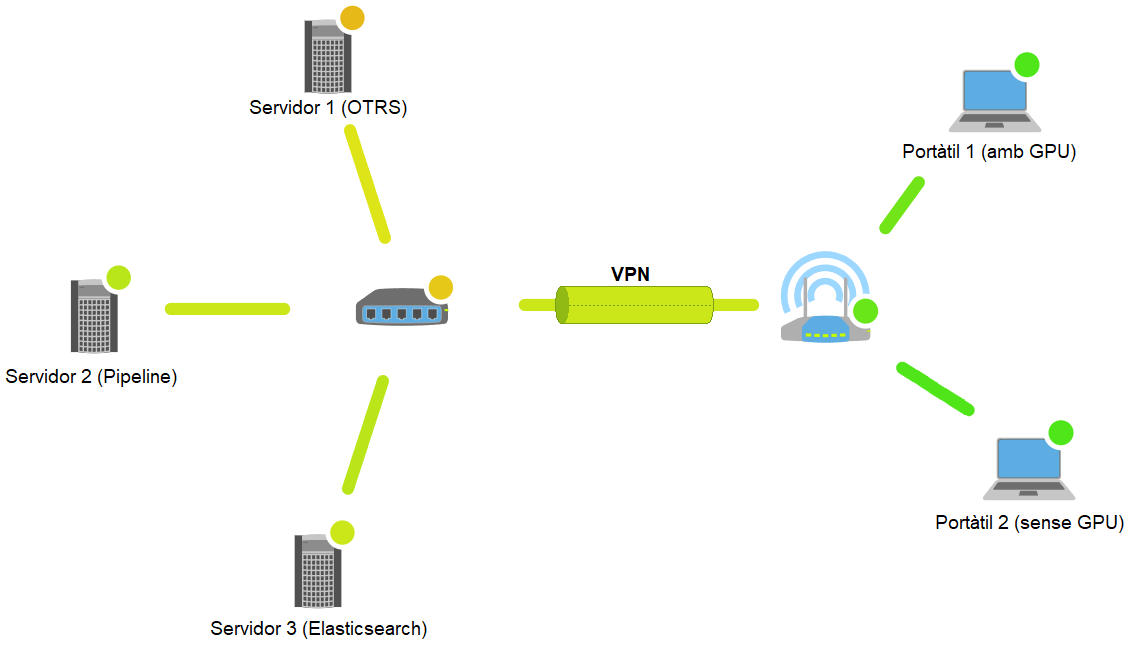
\includegraphics[width=0.8\textwidth]{network.png}
     \caption{Diagrama de la xarxa del projecte. \\ (Creació pròpia amb recursos de \textbf{yWorks})}
     \label{fig:network}
\end{figure}

El sistema consta d'una sèrie de scripts de Python que s'executen seqüencialment i duen a terme les tasques següents:

\begin{enumerate}
     \item Extreure els tiquets de la base de dades OTRS de l'\textbf{Agència}.
     \item Preprocessar el text de cada tiquet, eliminant el soroll, normalitzant el format i inserint les referències necessàries.
     \item Aplicar un model de processament del llenguatge natural (NLP) que detecta i extreu els camps rellevants de cada tiquet.
     \item Anonimitzar els camps extrets mitjançant una funció proporcionada per l'\textbf{Agència}, que substitueix les dades personals o sensibles per símbols o etiquetes genèriques.
     \item Emmagatzemar els camps anonimitzats en una base de dades Elasticsearch, que és un motor de cerca i anàlisi distribuïda.
\end{enumerate}

La figura \ref{fig:pipeline} mostra un diagrama de flux que il·lustra el funcionament del sistema.

\begin{figure}[H]
     \centering
     \vspace{1cm} % Adjust the vertical space (padding) at the top
     \setlength{\fboxsep}{5pt} % Adjust the padding
     \setlength{\fboxrule}{0pt} % Adjust the border thickness   
     \fbox{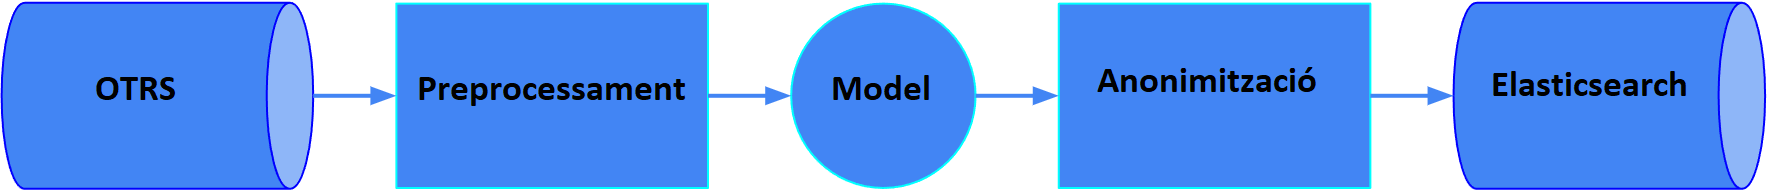
\includegraphics[width=0.8\textwidth]{pipeline.png}}
     \caption{Diagrama de flux del sistema d'anàlisi automàtica de tiquets d'incidències de ciberseguretat. \\ (Creació pròpia)}
     \label{fig:pipeline}
\end{figure}

En les següents seccions es detallen els components i les tecnologies utilitzades a cadascuna de les etapes del \textit{pipeline}.
\subsection{Extracció de tiquets d'OTRS}
% Explicar com està configurat el OTRS
% Explicar quines funcions es criden, com s'extreu del excel i les excepcions
% L'explicació dels tiquets es fa a l'apartat exploració teòrica
Per extreure els tiquets del Servidor OTRS de l'\textbf{Agència}, es fa servir \textit{PyOTRS}, que permet accedir a les dades mitjançant peticions amb la REST API. S'ha implementat un script de Python que utilitza la llibreria mencionada per fer les peticions i obtenir els tiquets. L'script s'encarrega d'autenticar-se amb les credencials cedides per l'\textbf{Agència}, extreure els tiquets especificats a un fitxer Excel i fer un post processament per obtenir tota l'informació del tiquet en un format estandaritzat i sense repeticions innecesàries. A continució es detalla el funcionament del codi seguint l'ordre que recorren els tiquets.

\begin{enumerate}
     \item \textbf{Iniciar sessió:} Es fan unes configuracions per assegurar que els tiquets es reben amb el format esperat i mitjançant les funcions creades a OTRS. Després es crea un client amb la adreça IP del servidor, el usuari i la contrassenya obtinguts de l'\textbf{Agència}.
     \item \textbf{Iterar pels tiquets:} Es busca i s'obra el fitxer excel especificat en el qual hi haurà l'informació necessària dels tiquets que s'ha de processar. S'itera per la columna en la que es troben els identificadors del tiquets.
     \item \textbf{Llegir ID del tiquet:} Per cada fila, es llegeix l'identificador del tiquet i es crida a la següent funció.
     \item \textbf{Comprovar l'utilització del tiquet:} Abans de començar a extreure els tiquets, es comprova si el tiquet en qüestió ja ha sigut extret abans. Això es fa per evitar cicles infinits amb referències cícliques dins dels tiquets. Es reinicia la llist a de tiquets visitats després de cada iteració.
     \item \textbf{Extreure tiquet:}
     \item \textbf{Processament del tiquet:}
     \item \textbf{Iterar pels articles:}
     \item \textbf{Processament del cos:}
     \item \textbf{Processament dels adjunts:}
     \item \textbf{Processament de les referències:}
     \item \textbf{Unir i retornar:}
\end{enumerate}


\subsection{Preprocessament de tiquets}
% Explicar quins apartats s'afegeixen als tiquets i quins es queden fora
% Quins attachments s'ha decidit utilitzar
% Com es busquen les referències
% Com s'organitza el tiquet amb els tres anteriors apartats (posar imatge/exemple)
\begin{comment}
     El preprocessament dels tiquets té com a objectiu preparar el text per analitzar-lo pel model de PLN. S'ha implementat un script de Python que realitza les operacions següents sobre el text de cada tiquet:

\begin{itemize}
     \item Eliminar els elements HTML, les capçaleres, les signatures i els missatges anteriors que puguin contenir els tiquets, ja que no aporten informació rellevant per a l'anàlisi.
     \item Normalitzar el text, convertint totes les lletres a minúscules, eliminant els signes de puntuació, els números i els caràcters especials, i substituint els espais múltiples per un de sol.
     \item Tokenitzar el text, és a dir, dividir-lo en unitats mínimes de significat, que en aquest cas són les paraules. S'ha utilitzat la llibreria NLTK per fer aquesta tasca, que ofereix diferents algorismes de tokenització per a diferents idiomes.
\end{itemize}

El resultat del preprocessament és una llista de tokens per cada tiquet, que s'emmagatzema en un altre fitxer local per a la seva posterior anàlisi.
\end{comment}

\subsection{Aplicació del model NLP}
\begin{comment}

Per aplicar el model de PLN que detecta i extreu els camps rellevants de cada tiquet, s'ha fet servir la llibreria spaCy, que és un framework de codi obert per al processament del llenguatge natural. SpaCy ofereix diversos models preentrenats per a diferents idiomes, que permeten fer tasques com l'anàlisi sintàctica, l'etiquetació morfològica, l'extracció d'entitats nomenades, la classificació de textos, etc.

En aquest cas, s'ha utilitzat el model preentrenat per a l'espanyol, que s'anomena \\ $es_core\_news\_sm$. Aquest model és capaç de reconèixer les entitats anomenades següents: persona, organització, lloc, producte, esdeveniment, obra d'art, llei, data, hora, percentatge, diners, quantitat, ordinal i cardinal. Tot i això, no totes aquestes entitats són rellevants per a l'anàlisi dels tiquets d'incidències de ciberseguretat, ia més hi ha alguns camps que no es corresponen amb cap d'aquestes entitats, com el tipus d'incidència o el nivell de prioritat.

Per tant, s'ha realitzat un procés d'adaptació del model preentrenat, que consisteix a afegir noves entitats i reentrenar el model amb un conjunt de dades etiquetat específicament per al domini dels tiquets de ciberseguretat. El conjunt de dades etiquetatge s'ha obtingut a partir d'una mostra de tiquets reals de l'Agència, que s'han anotat manualment amb les entitats següents:

\begin{itemize}
     \item TIPUS: el tipus d'incidència, que pot ser phishing, malware, ransomware, atac DDoS, etc.
     \item PRIORITAT: el nivell de prioritat assignat al tiquet, que pot ser baixa, mitjana, alta o crítica.
     \item USUARI: nom o àlies de l'usuari afectat per la incidència.
     \item DISPOSITIU: el nom o l'adreça IP del dispositiu compromès per la incidència.
     \item DATA: la data en què es va produir o es va reportar la incidència.
     \item HORA: l'hora en què es va produir o es va reportar la incidència.
     \item ORG: l'organització a què pertany l'usuari o dispositiu afectat, que es manté com una entitat preexistent del model.
     \item LOC: el lloc des del qual es va originar o detectar la incidència, que es manté com una entitat preexistent del model.
\end{itemize}

El procés d'adaptació del model s'ha realitzat seguint els passos descrits a la documentació de spaCy, que consisteixen en:

\begin{enumerate}
     \item Crear un objecte de la classe Language a partir del model preentrenat.
     \item Afegir les noves entitats al component de reconeixement d'entitats nomenades (NER) del model, mitjançant el mètode add\_label.
     \item Deshabilitar els altres components del model, com l'analitzador sintàctic o l'etiquetador morfològic, ja que no es faran servir i poden interferir amb l'entrenament del NER.
     \item Crear un objecte de classe EntityRecognizer a partir del component NER del model, i assignar-li un optimitzador, una funció de pèrdua i unes mètriques d'avaluació.
     \item Entrenar l'objecte EntityRecognizer amb el conjunt de dades etiquetatge, mitjançant el mètode update, que rep com a paràmetres els textos i les anotacions de les entitats, i torna la pèrdua i les mètriques a cada iteració.
     \item Desar el model adaptat en un fitxer local, mitjançant el mètode to\_disk.
\end{enumerate}

El resultat de l'entrenament és un model de PLN capaç de detectar i extreure els camps rellevants dels tiquets d'incidències de ciberseguretat, que s'aplica a cada tiquet preprocessat i s'emmagatzema el resultat en un altre fitxer local per a la seva posterior anonimització.
\end{comment}

\subsection{Anonimització de camps}

\begin{comment}
L'anonimització dels camps extrets té com a objectiu protegir la privadesa i la confidencialitat de les dades personals o sensibles que puguin contenir els tiquets d'incidències de ciberseguretat. Per fer-ho, s'ha utilitzat una funció proporcionada per l'Agència, que rep com a paràmetre el text d'un camp i torna un text anonimitzat, que substitueix les dades per símbols o etiquetes genèriques. Per exemple, si el text del camp és "Juan Pérez", la funció torna "NOM COGNOM", i si el text és "192.168.1.1", la funció torna "IP PRIVADA".

La funció d'anonimització s'ha implementat en un script de Python que rep com a entrada el fitxer amb els camps extrets pel model de PLN, i torna com a sortida un altre fitxer amb els camps anonimitzats, que s'emmagatzemen en un diccionari amb la següent estructura:
\end{comment}

\subsection{Emmagatzematge del resultat}
